\documentclass[a4paper, 10pt]{article}
\usepackage[utf8]{inputenc}
%\usepackage[brazil]{babel}
\usepackage[top=3cm,left=3cm,right=2cm,bottom=2cm]{geometry} % para as margens
\usepackage{graphicx} % para as figuras  
\usepackage{color}
\usepackage[hidelinks]{hyperref}
\usepackage{listings}

\newcommand{\ee}{Enactment Engine}
\newcommand{\cd}{Choreography Deployer}
\newcommand{\dm}{Deployment Manager}

\title{CHOReOS \ee\ Installation Guide}
\author{Leonardo Leite (IME - USP)}

\begin{document}

\maketitle

\section{Introduction}

The CHOReOS \ee\ provides a Platform as a Service (PaaS) that automates the distributed deployment of service choreographies in cloud environments. This document provides instructions about how to install, configure, and run the \ee.

The \ee\ is composed by the components pictured on Figure~\ref{img:ee_components}, from which \cd\ and \dm\ are provided by the \ee, whereas the Chef components and the Cloud Gateway are third-party used by the \ee.

\begin{figure}
\centering
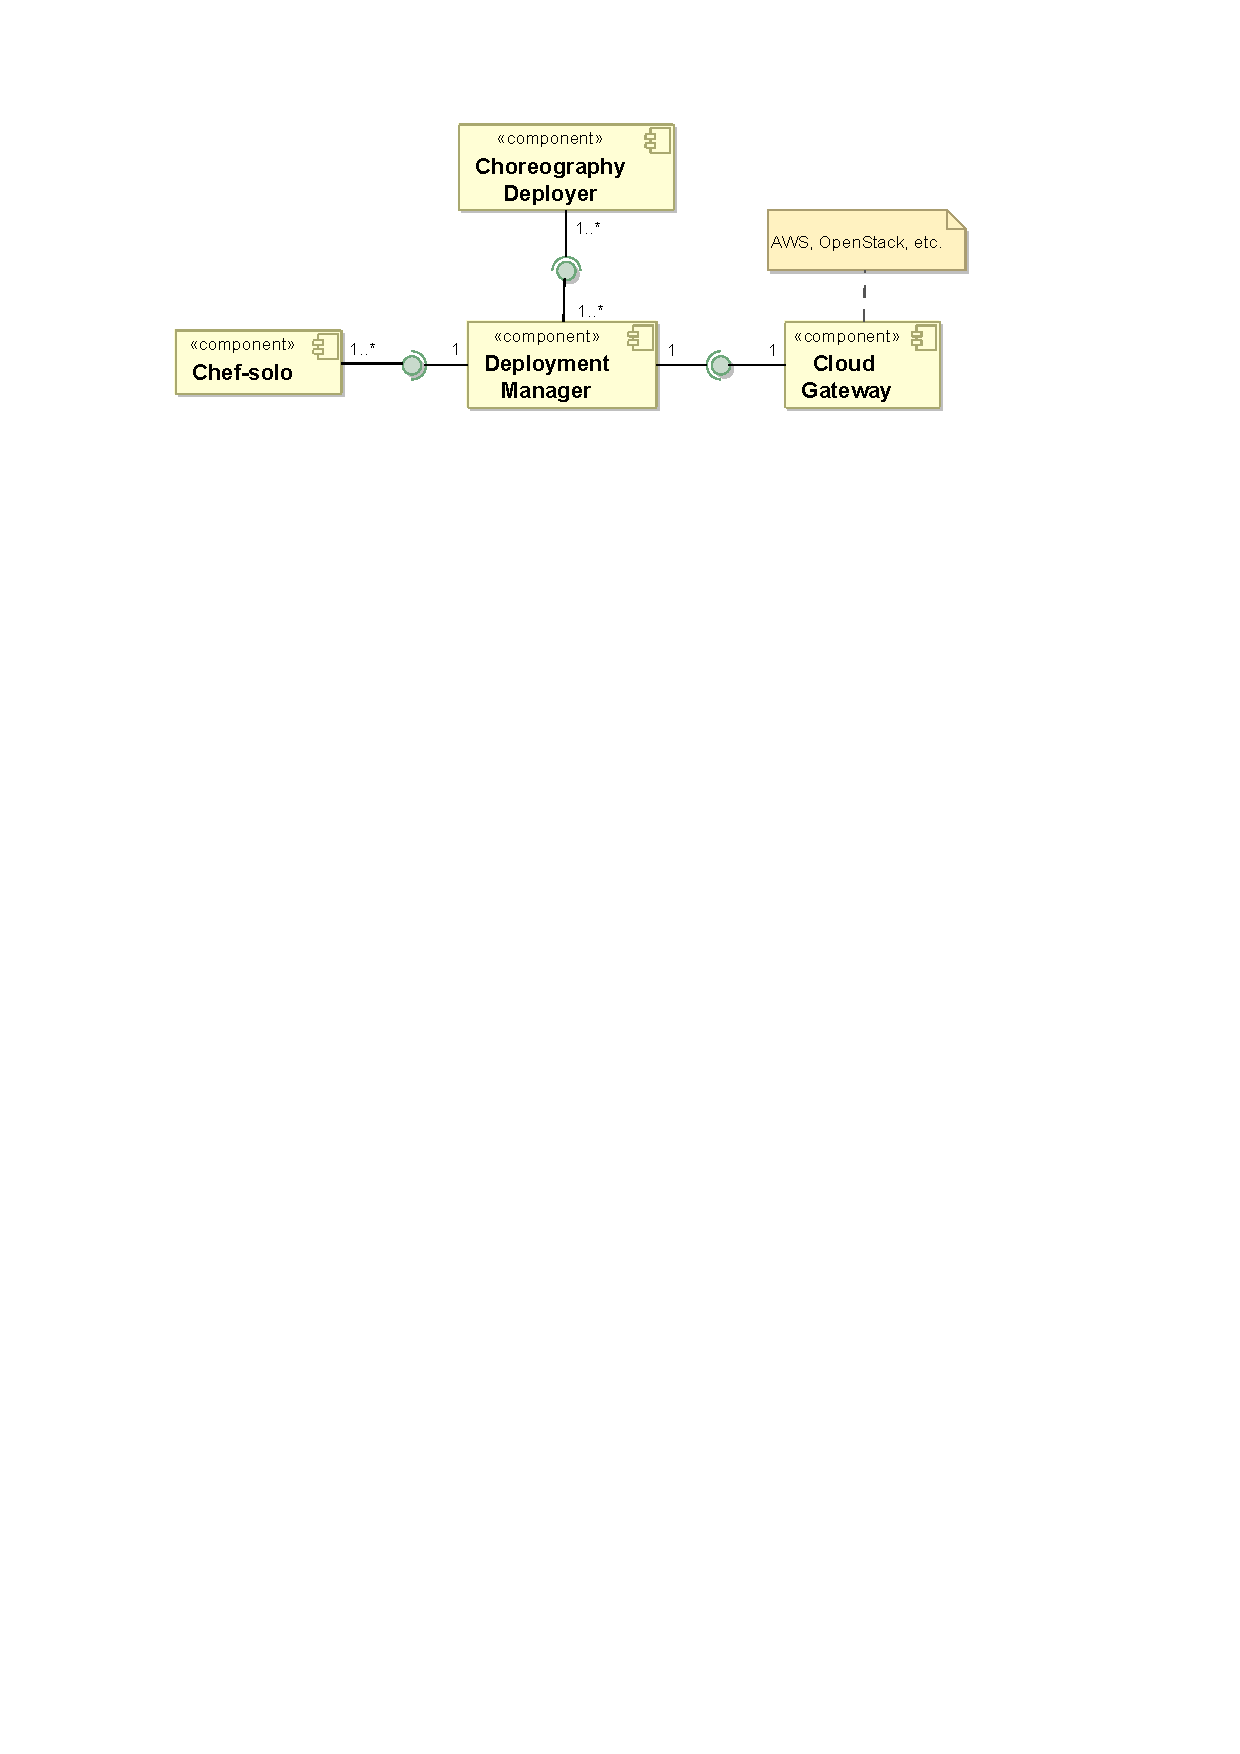
\includegraphics[scale=0.7]{img/components.pdf}
\caption{\ee\ architecture}
\label{img:ee_components}
\end{figure}

In this guide we assume that both \cd\ and \dm\ components will be executed on the deployer machine. Deployer is the human operator responsible by the deployment process. For while, a \cd\ instance is limited to use only one \dm.

\section{Requirements}

Before you run \ee, you will need:

\begin{itemize}
\item SVN;
\item Java 6 (we are using OpenJDK);
\item Maven 3  (\url{http://maven.apache.org/download.html});
\item a Cloud Gateway access, as detailed in Section~\ref{sec:cloud};
\item a Chef account, as detailed in Section~\ref{sec:chef}.
\end{itemize}

\section{Cloud Gateway}
\label{sec:cloud}

\subsection{Amazon EC2}

\subsection{OpenStack}

\subsection{Fixed cloud provider}

\section{Chef}
\label{sec:chef}

\dm\ will properly configure the nodes using Chef, an open-source configuration management system. With Chef you can specify a resources set to be deployed into cloud nodes. These resources are described by a Ruby-like DSL (Domain Specific Language), and include: systems, files, scripts execution, and others.

You can setup your own Chef server, or create an Hosted Chef server account. Hosted Chef is offered by Opscode\footnote{\url{http://www.opscode.com/}}. Although Hosted Chef frees you from setting the Chef Server in the infrastructure of your organization, it allows only a limited number of nodes to be managed by Chef.

Make sure your \texttt{knife.rb} file be something like the example on Listing~\ref{lst:kniferb}.

{\footnotesize
\begin{lstlisting}[caption=knife.rb example,label=lst:kniferb] 
%log_level                :info 
%log_location             STDOUT 
%node_name                "lleite" 
%client_key               "#{current_dir}/lleite.pem" 
%validation_client_name   "choreos-verao-validator" 
%validation_key           "#{current_dir}/choreos-verao-validator.pem" 
%chef_server_url          "https://api.opscode.com/organizations/choreos-verao" 
%cache_type               'BasicFile' 
%cache_options( :path => "#{ENV['HOME']}/.chef/checksums" ) 
%cookbook_path            ["#{current_dir}/../cookbooks"] 
\end{lstlisting}
}

Here, "lleite" is also my Opscode user name, and "choreos-verao" is the organization name configured on Hosted Chef. And don't forget the "cookbook\_path" property.

You will also need to upload to your Chef Server all the cookbooks from our cookbook folder: https://github.com/choreos/choreos\_middleware/tree/master/chef-repo/cookbooks.


\section{Checkout and Compilation}

To checkout the code: \texttt{svn checkout http://ow2.forge \dots}

After installing Maven 3, open the terminal at the \texttt{choreos\_middleware} folder, and run the \texttt{build.sh} script. It can take several minutes. Internet access is necessary during compilation.

\section{Configuration}

Open the folder \texttt{DeploymentManager/src/main/resources}, and create a \texttt{deployment.properties} file by copying the \texttt{deployment.properties.template} file. The new properties file must be created in the same folder.

Open the just created properties file and edit it following instructions on the template file. The Listing~\ref{lst:deployment_properties} shows an example.

\lstset{
numbers=left
}

{\footnotesize
\begin{lstlisting}[caption=deployment.properties example,label=lst:deployment_properties] 
NODE_POOL_MANAGER_PORT=9100
SERVICE_DEPLOYER_PORT=9101
NODE_SELECTOR=ROUND_ROBIN
CLOUD_PROVIDER=AWS
FIXED_VM_IP=192.168.56.102
FIXED_VM_HOSTNAME=choreos-node
FIXED_VM_PRIVATE_SSH_KEY=/home/leonardo/.ssh/nopass
FIXED_VM_USER=choreos
AMAZON_ACCESS_KEY_ID=AKIAIIT213ISasdSECRETEFJH6Q
AMAZON_SECRET_KEY=N+KzHQITasdIS123ALSOwzAj9MiSECRETE0UPuwyD
AMAZON_KEY_PAIR=leofl
AMAZON_PRIVATE_SSH_KEY=/home/leonardo/.ssh/leofl.pem
CHEF_CONFIG_FILE=/home/leonardo/chef/chef-repo/.chef/knife.rb
CHEF_REPO=/home/leonardo/chef/chef-repo
\end{lstlisting}
}

NODE\_SELECTOR options...


\section{Execution}

After compiling the project, to run both \cd\ and \dm\ you have just to run the main method, on the following classes: \textsf{org.ow2.choreos.deployment.rest.DeploymentManagerServer} and \textsf{org.ow2.choreos.chors.rest.ChorDeployerServer}.

This task can be easier accomplished if you import the \ee\ projects in the Eclipse IDE. After importing the project, open the menu \texttt{Window>>Preferences>>Java>>Build Path>>Classpath} variables, and set the \texttt{M2\_REPO} variable pointing to your Maven repository folder, usually the \texttt{.m2/repository} folder within your home folder. Obs: we have used the Eclipse Indigo version.

If you successfully start the \cd\ and the \dm\, you must see the following messages on their respective consoles: 

\texttt{\cd\ has started [http://localhost:9100/choreographydeployer/]}

\texttt{\dm\ has started [http://localhost:9101/deploymentmanager/]}

To verify if it is everything OK, run the \textsf{org.ow2.choreos.chors.SimpleChorEnactmentTest}. This test will deploy a simple choreography composed of two services and try to invoke it.



\end{document}
